\documentclass{beamer}


\usepackage[utf8]{inputenc}
\usepackage[italian]{babel}
\usepackage{listings}
\usepackage{xcolor}


\usetheme{Madrid}
\usecolortheme{orchid}


\definecolor{codegray}{rgb}{0.5,0.5,0.5}      % grigio
\definecolor{codeorange}{rgb}{0.6, 0.2, 0.0}  % arancione
\definecolor{codegreen}{rgb}{0, 0.4, 0}       % verde

\newcommand{\highlightorange}[1]{{\color{codeorange}#1}}
\newcommand{\highlightgreen}[1]{{\color{codegreen}#1}}

\lstset{
    literate=%
    {à}{{\`a}}1
    {è}{{\`e}}1
    {ì}{{\`i}}1
    {ò}{{\`o}}1
    {ù}{{\`u}}1
    {á}{{\'a}}1
    {é}{{\'e}}1
    {í}{{\'i}}1
    {ó}{{\'o}}1
    {ú}{{\'u}}1
    {À}{{\`A}}1
    {È}{{\`E}}1
    {Ì}{{\`I}}1
    {Ò}{{\`O}}1
    {Ù}{{\`U}}1
    {Á}{{\'A}}1
    {É}{{\'E}}1
    {Í}{{\'I}}1
    {Ó}{{\'O}}1
    {Ú}{{\'U}}1
}

\lstset{
    commentstyle=\color{codegray},    % colore commenti: grigio
    keywordstyle=\color{codeorange},  % colore parole chiave: arancione
    stringstyle=\color{codegreen},    % colore stringhe: verde
    basicstyle=\ttfamily\footnotesize,       % Imposta il font monospazio di dimensione piccola
    showspaces=false,                 % Non mostra gli spazi
    showtabs=false,                   % Non mostra i tab
    showstringspaces=false,           % Non mostra gli spazi nelle stringhe
    frame=none,                       % Aggiunge una cornice attorno al codice
    tabsize=4,                        % Imposta la dimensione del tab a 2 spazi
    keepspaces=true,                  % Mantiene gli spazi nel testo
    columns=flexible,                 % Colonne flessibili
    numbers=none,                     % Mostra i numeri di riga a sinistra
    numbersep=5pt,                    % Distanza tra i numeri di riga e il codice
}


\title{
    {\Huge TooDY}\\
    {\small a Tool for Detecting variabilitY}}
\author{
    Matteo Giorgi
    \vspace{3mm}
}
\institute{
    % 
\includegraphics[width=2cm]{cherubino.png}\\
    % \vspace{3mm}
    Università degli Studi di Pisa
    \vspace{-3mm}
}
\date{
    \tiny 01 Dicembre 2023\\
    \vspace{5mm}
    
\includegraphics[width=1.5cm]{cherubino.png}
}
% \logo{
\includegraphics[height=1.5cm]{cherubino.png}}


\setbeamertemplate{navigation symbols}{}




\begin{document}
\setbeamertemplate{footline}{
    \leavevmode%
    \hbox{%
        \begin{beamercolorbox}[wd=.3333\paperwidth,ht=2.25ex,dp=1ex,center]{author in head/foot}
        \usebeamerfont{author in head/foot}Matteo Giorgi
        \end{beamercolorbox}%
        \begin{beamercolorbox}[wd=.6667\paperwidth,ht=2.25ex,dp=1ex,right]{title in head/foot}
        \usebeamerfont{title in head/foot}TooDY, a Tool for Detecting variabilitY\hfill\insertframenumber{} / \inserttotalframenumber\hspace*{2ex}
        \end{beamercolorbox}%
    }%
    \vskip0pt%
}


\begin{frame}
\titlepage
\end{frame}
% \logo{}


\begin{frame}
\frametitle{Software Product Lines \& Variabilità}

\begin{columns}
\column{0.95\textwidth}
\begin{alertblock}{Scopo del Progetto}
Realizzare uno strumento di elaborazione del linguaggio naturale, per individuare indicatori di variabilità in un documento dei requisiti.
\end{alertblock}
Il progetto implementa una web-app \textbf{Flask}, che esegue analisi lessicale e sintattica, con il supporto della libreria open-source \textbf{spaCy}.
\end{columns}

\begin{columns}
\column{0.45\textwidth}
\begin{block}{SPL Engineering}
È un paradigma di sviluppo software che modella le caratteristiche comuni e quelle di variabilità di una famiglia di sistemi correlati, al fine di massimizzare il riutilizzo e ridurre i costi di sviluppo.
\end{block}
\column{0.45\textwidth}
\begin{block}{Variabilità in un requisito}
Rappresenta la capacità del requisito stesso di corrispondere a più di una possibile configurazione e di essere modificato o esteso a seconda del contesto specifico in cui viene implementato.
\end{block}
\end{columns}
\end{frame}


\begin{frame}
\frametitle{Indicatori di Variabilità}

I \textbf{difetti di ambiguità} nei requisiti possono fornire un’indicazione di variabilità (in design, implementazione o configurabilità).

\vspace{0.25cm}
\begin{itemize}
\item \textbf{Vaghezza} -- parole con significato non quantificabile o univoco.
\item \textbf{Debolezza} -- presenza di un verbo debole (non imperativo).
\item \textbf{Forma passiva} -- ambigua se non è chiaro chi compie l'azione.
\item \textbf{Opzionalità} -- presenza di parole come \textit{possibly} o \textit{probably}.
\item \textbf{Molteplicità} -- riferimento a una pluralità di oggetti (\textit{and}, \textit{or}).
\item \textbf{If, When, Where} -- clausole subordinate che indicano condizioni.
\end{itemize}
\end{frame}


\begin{frame}
\frametitle{Caso di Studio: Coffee Vending-Machine}

\begin{columns}
\column{0.45\textwidth}
\begin{itemize}
\item[\textbf{R1.}] After inserting a \highlightgreen{suitable} coin, the user shall choose a beverage and select the amount of sugar.
\item[\textbf{R2.}] The machine shall offer, as beverages, coffee \highlightorange{and} cappuccino \highlightgreen{or} tea.
\item[\textbf{R3.}] The machine shall \highlightorange{always} offer coffee.
\end{itemize}
\column{0.45\textwidth}
\begin{itemize}
\item[\textbf{R4.}] A ringtone \highlightgreen{possibly} has to \highlightorange{be played} after beverage delivery.
\item[\textbf{R5.}] After the beverage \highlightorange{is taken}, the machine returns idle.
\item[\textbf{R6.}] The British market requires tea and excludes \highlightorange{any} ring tone.
\end{itemize}
\end{columns}

\begin{figure}
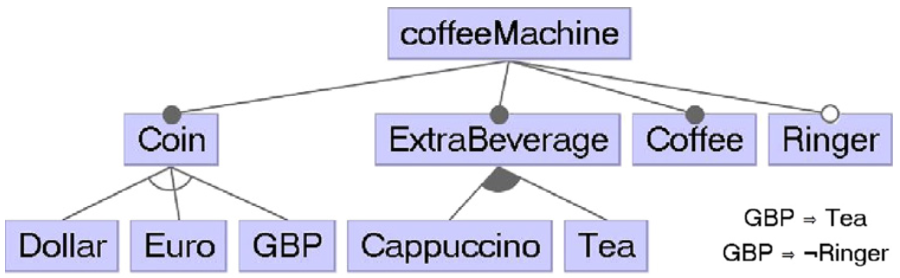
\includegraphics[width=0.7\textwidth]{coffee2.png}
% \caption{\textit{Feature Diagram} per la Coffee Vending-Machine.}
\end{figure}
\end{frame}


% \begin{frame}
% \frametitle{Feature Diagrams e il loro Ruolo in FODA}
% \begin{itemize}
% \item I \textbf{Feature Diagrams} sono strumenti chiave in \textit{Feature-Oriented Domain Analysis (FODA)}.
% \item Rappresentano visualmente le \textit{features} di un sistema e le loro relazioni.
% \item Aiutano a identificare e modellare la variabilità e le caratteristiche comuni in una SPL.
% \end{itemize}
% \end{frame}


\begin{frame}
\frametitle{Analisi del Linguaggio Naturale}

Dato un testo, l’\textbf{elaborazione del linguaggio naturale} prevede quattro fasi distinte per analizzarlo e comprenderlo.

\vspace{0.25cm}
\begin{enumerate}
\item \textbf{Tokenizzazione} -- Suddivide il testo in unità significative (\textit{token}).
\item \textbf{An.Morfologica} -- Identifica il ruolo dei \textit{token} nel discorso.
\item \textbf{An.Sintattica} -- Studia la struttura grammaticale del periodo.
\item \textbf{An.Semantica} -- Interpreta il significato delle strutture sintattiche.
\end{enumerate}

\begin{block}{Cos'è spaCy?}
È una libreria Python open-source per NLP, che offre parsing sintattico e semantico, tokenizzazione, PoS-Tagging, Named Entity Recognition, supporta modelli di apprendimento automatico e integrazione con TensorFlow e PyTorch.
\end{block}
\end{frame}


\begin{frame}[fragile]
\frametitle{Funzionalità di spaCy}

\begin{columns}
\column{0.45\textwidth}
\begin{enumerate}
\item Tokenizzazione
\item PoS-Tagging
\item Dependency Parsing
\item Lemmatizzazione
\end{enumerate}
\column{0.45\textwidth}
\begin{enumerate}
\item Sentence Boundary Detection
\item Named Entity Recognition
\item Rule-Based Matching
\end{enumerate}
\end{columns}

\vspace{0.25cm}
\begin{block}{Esempio di Rule-Based Matching con \texttt{Matcher}}
\begin{lstlisting}[language=Python]
import spacy
from spacy.matcher import Matcher

nlp = spacy.load("it_core_news_sm")
matcher = Matcher(nlp.vocab)
pattern = [{"POS": "NOUN"}, {"POS": "ADJ"}]
matcher.add("NOUN_ADJ_PATTERN", [pattern])

doc = nlp("Il mercato azionario ha mostrato una crescita costante.")
matches = matcher(doc)
\end{lstlisting}
\end{block}
\end{frame}


\begin{frame}
\frametitle{Parser lessicale}

\begin{figure}
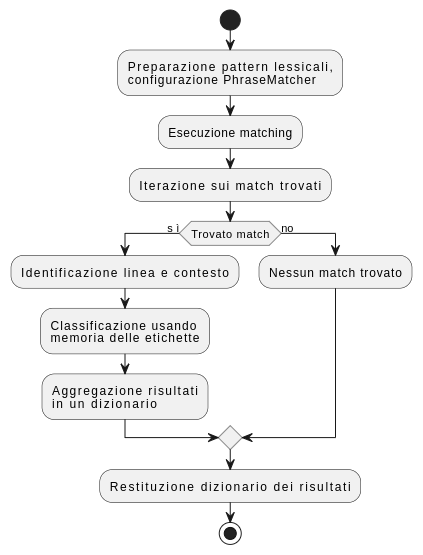
\includegraphics[width=0.5\textwidth]{lexical_analyser.png}
\end{figure}
\end{frame}


\begin{frame}[fragile]
\frametitle{Parser forma passiva}

\begin{lstlisting}[language=Python]
import spacy
from spacy.matcher import Matcher

nlp = spacy.load("it_core_news_sm")
matcher = Matcher(nlp.vocab)
pattern = [{"POS": "NOUN"}, {"POS": "ADJ"}]
matcher.add("NOUN_ADJ_PATTERN", [pattern])

doc = nlp("Il mercato azionario ha mostrato una crescita costante.")
matches = matcher(doc)
\end{lstlisting}
\end{frame}


\begin{frame}[fragile]
\frametitle{Parser di congiunzioni verbali}

\begin{lstlisting}[language=Python]
import spacy
from spacy.matcher import Matcher

nlp = spacy.load("it_core_news_sm")
matcher = Matcher(nlp.vocab)
pattern = [{"POS": "NOUN"}, {"POS": "ADJ"}]
matcher.add("NOUN_ADJ_PATTERN", [pattern])

doc = nlp("Il mercato azionario ha mostrato una crescita costante.")
matches = matcher(doc)
\end{lstlisting}
\end{frame}


\begin{frame}[fragile]
\frametitle{Analizzatore di condizioni}

\begin{lstlisting}[language=Python]
import spacy
from spacy.matcher import Matcher

nlp = spacy.load("it_core_news_sm")
matcher = Matcher(nlp.vocab)
pattern = [{"POS": "NOUN"}, {"POS": "ADJ"}]
matcher.add("NOUN_ADJ_PATTERN", [pattern])

doc = nlp("Il mercato azionario ha mostrato una crescita costante.")
matches = matcher(doc)
\end{lstlisting}
\end{frame}
\end{document}
